\clearpage

\section{Binary Source}

\begin{tcolorbox}	
	\begin{tabular}{p{2.75cm} p{0.2cm} p{10.5cm}} 	
		\textbf{Header File}   &:& binary\_source.h \\
		\textbf{Source File}   &:& binary\_source.cpp \\
	\end{tabular}
\end{tcolorbox}

\maketitle
This block generates a sequence of binary values (1 or 0) and it can work in four different modes:

\begin{multicols}{2}
\begin{enumerate}
	\item Random
	\item PseudoRandom
	\item DeterministicCyclic
	\item DeterministicAppendZeros
\end{enumerate}
\end{multicols}

This blocks doesn't accept any input signal. It produces any number of output signals.

\subsection*{Input Parameters}

%	\begin{itemize}
%		\item mode\{PseudoRandom\}\linebreak
%		(Random, PseudoRandom, DeterministicCyclic, DeterministicAppendZeros)
%		\item probabilityOfZero\{0.5\}\linebreak
%		(real $\in$ [0,1])
%		\item patternLength\{7\} \linebreak
%		(integer $\in$ [1,32])
%		\item bitStream\{"0100011101010101"\} \linebreak
%		(string of 0's and 1's)
%		\item numberOfBits\{-1\} \linebreak
%		(long int)
%		\item bitPeriod\{1.0/100e9\} \linebreak
%		(double)
%	\end{itemize}

\begin{table}[h]
	\centering
	\begin{tabular}{|c|c|p{60mm}|c|ccp{60mm}}
		\cline{1-4}
		\textbf{Parameter} & \textbf{Type} & \textbf{Values} &   \textbf{Default}& \\ \cline{1-4}
		mode & string & Random, PseudoRandom, DeterministicCyclic, DeterministicAppendZeros & PseudoRandom \\ \cline{1-4}
		probabilityOfZero & real & $\in$ [0,1] & 0.5 \\ \cline{1-4}
		patternLength & int &  Any natural number & 7 \\ \cline{1-4}
		bitStream & string & sequence of 0's and 1's & 0100011101010101 \\ \cline{1-4}
		numberOfBits & long int & any & -1 \\ \cline{1-4}
		bitPeriod & double & any & $1.0/100e9$ \\ \cline{1-4}
	\end{tabular}
	\caption{Binary source input parameters}
	\label{table:bin_sour_in_par}
\end{table}

\subsection*{Methods}

BinarySource(vector$\langle$Signal *$\rangle$ \&InputSig, vector$\langle$Signal *$\rangle$ \&OutputSig) :Block(InputSig, OutputSig)\{\};
\bigbreak	
void initialize(void);
\bigbreak	
bool runBlock(void);
\bigbreak	
void setMode(BinarySourceMode m)
BinarySourceMode const getMode(void)
\bigbreak	
void setProbabilityOfZero(double pZero)
\bigbreak
double const getProbabilityOfZero(void)
\bigbreak	
void setBitStream(string bStream)
\bigbreak
string const getBitStream(void)
\bigbreak	
void setNumberOfBits(long int nOfBits)
\bigbreak
long int const getNumberOfBits(void)
\bigbreak	
void setPatternLength(int pLength)
\bigbreak
int const getPatternLength(void)
\bigbreak	
void setBitPeriod(double bPeriod)
\bigbreak
double const getBitPeriod(void)

\subsection*{Functional description}

The \textit{mode} parameter allows the user to select between one of the four operation modes of the binary source.

\subparagraph*{Random Mode}
Generates a 0 with probability \textit{probabilityOfZero} and a 1 with probability 1-\textit{probabilityOfZero}.

\subparagraph*{Pseudorandom Mode}
Generates a pseudorandom sequence with period $2^\textit{patternLength}-1$.

\subparagraph*{DeterministicCyclic Mode}
Generates the sequence of 0's and 1's specified by \textit{bitStream} and then repeats it.

\subparagraph*{DeterministicAppendZeros Mode}
Generates the sequence of 0's and 1's specified by \textit{bitStream} and then it fills the rest of the buffer space with zeros.

\subsection*{Input Signals}


\subparagraph*{Number:} 0

\subparagraph*{Type:} Binary (DiscreteTimeDiscreteAmplitude)

\subsection*{Output Signals}

\subparagraph*{Number:} 1 or more

\subparagraph*{Type:} Binary (DiscreteTimeDiscreteAmplitude)

\subsection*{Examples}

\paragraph*{Random Mode}

\paragraph*{PseudoRandom Mode}
As an example consider a pseudorandom sequence with \textit{patternLength}=3 which contains a total of 7 ($2^3-1$) bits. In this sequence it is possible to find every combination of 0's and 1's that compose a 3 bit long subsequence with the exception of $000$. For this example the possible subsequences are $010$, $110$, $101$, $100$, $111$, $001$ and $100$ (they appear in figure \ref{BinarySequenceN3} numbered in this order). Some of these require wrap.

\begin{figure}[h]
	\centering
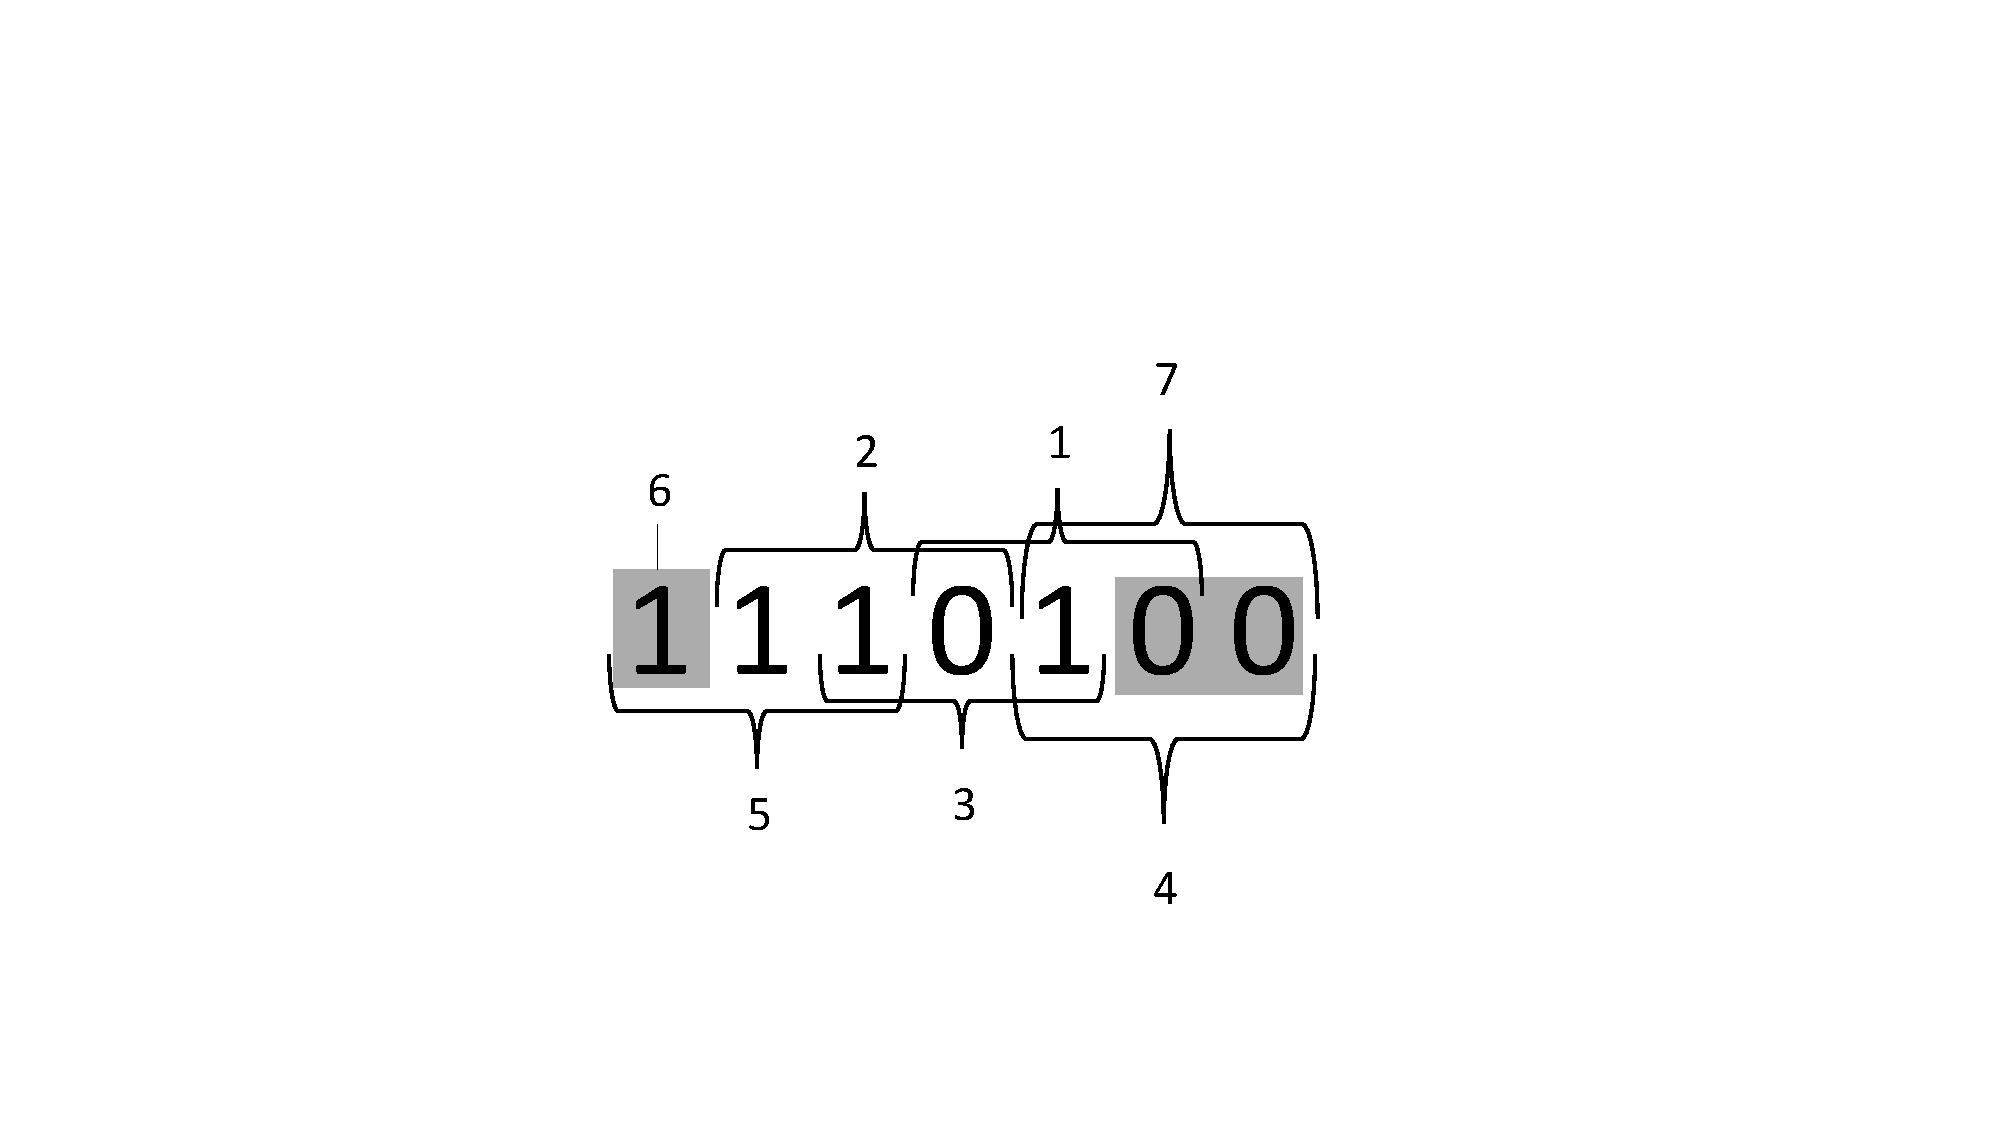
\includegraphics[width=\textwidth]{./lib/binary_source/figures/BinarySequenceN3.pdf}
\caption{Example of a pseudorandom sequence with a pattern length equal to 3.}\label{BinarySequenceN3}
\end{figure}

\paragraph*{DeterministicCyclic Mode}

As an example take the \textit{bit stream} '0100011101010101'. The generated binary signal is displayed in.

\paragraph*{DeterministicAppendZeros Mode}

Take as an example the \textit{bit stream} '0100011101010101'. The generated binary signal is displayed in \ref{MQAM1_DeterministAppendZeros}.

\begin{figure}
	\centering
	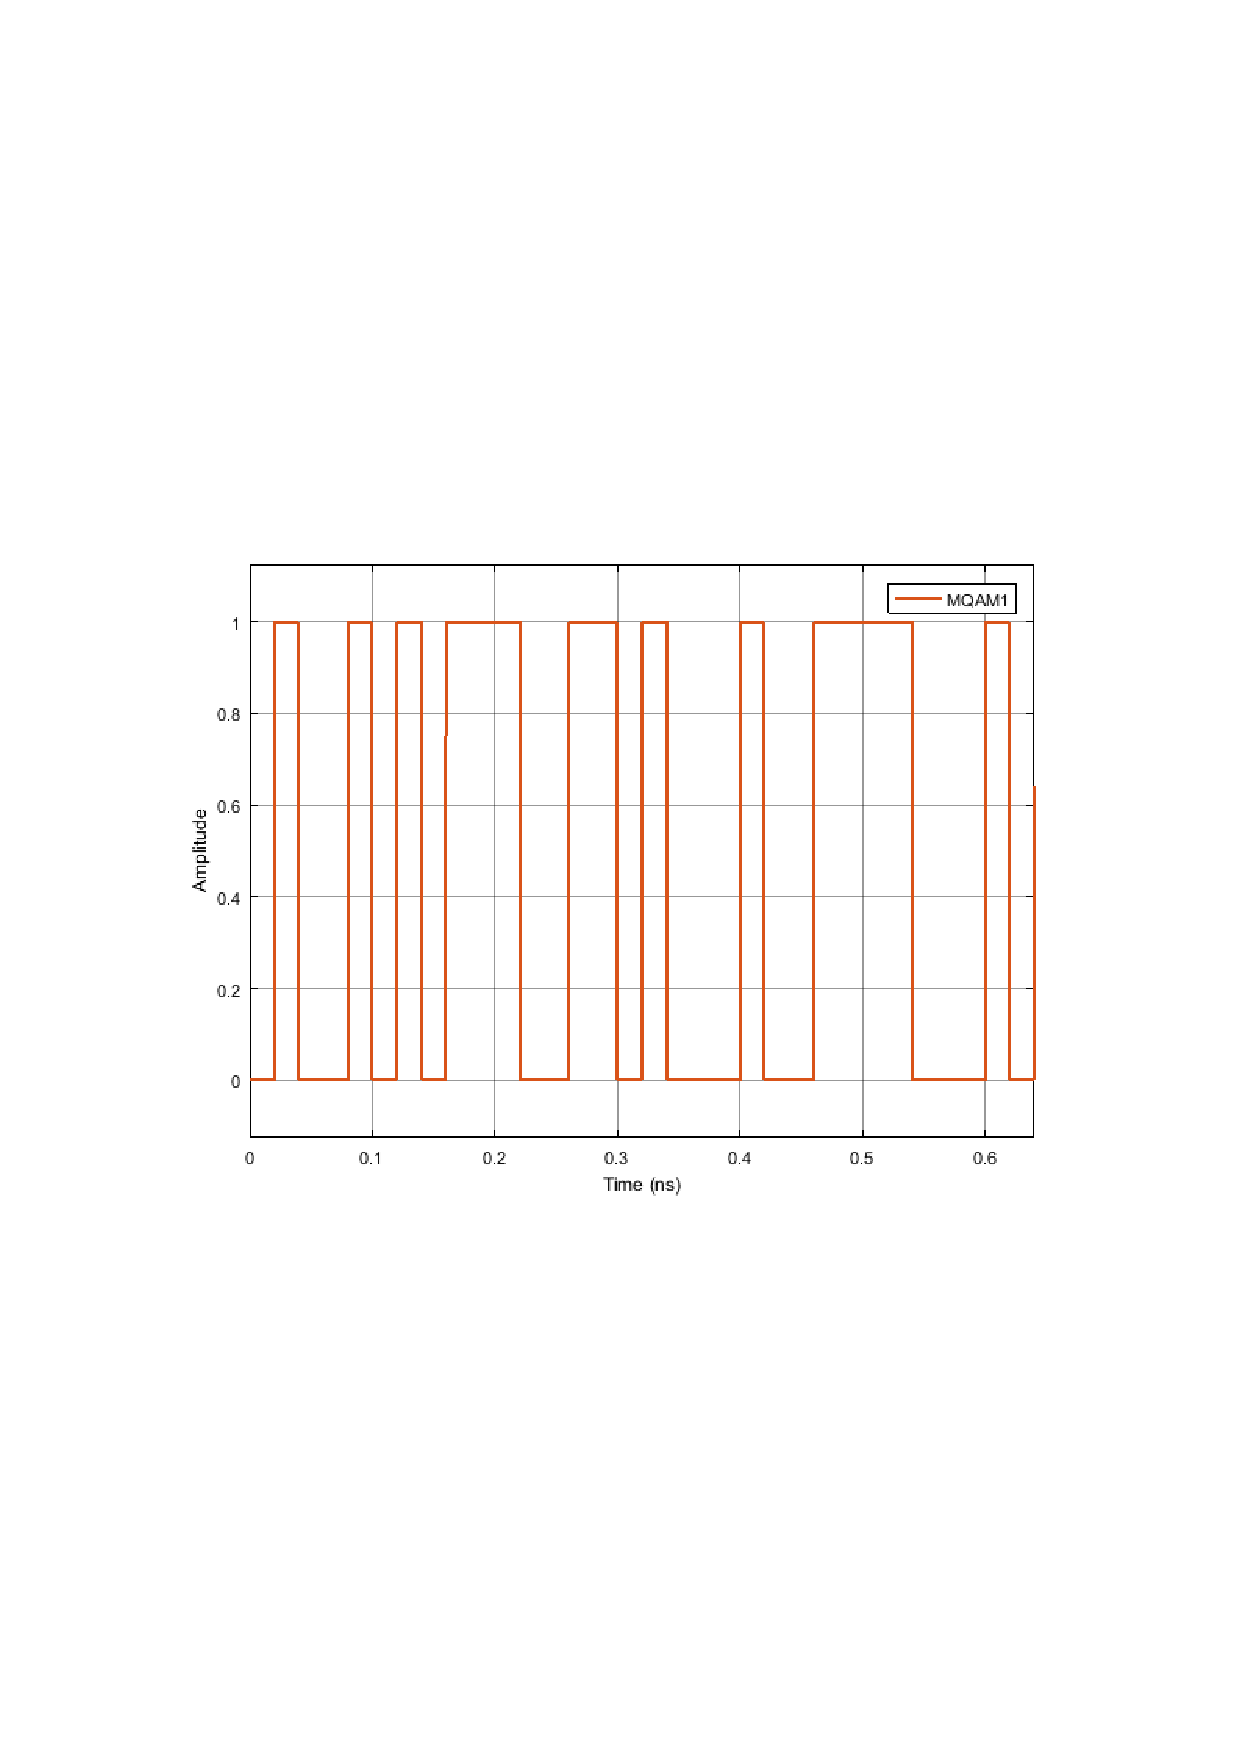
\includegraphics[clip, trim=0.5cm 9cm 0.5cm 9cm, width=\textwidth]{./lib/binary_source/figures/BinarySource_output.pdf}
	
	\caption{Binary signal generated by the block operating in the \textit{Deterministic Append Zeros} mode with a binary sequence 01000...}\label{MQAM1_DeterministAppendZeros}
\end{figure}

\subsection*{Sugestions for future improvement}

Implement an input signal that can work as trigger.

